\chapter{Toroidal Rectangle Network}
\label{Chap:Numerical}
\section{Toroidal Rectangle Network Notions}
The toroidal network is a regular complex in that each polygonal face has the same number of links and each node is connected to the same number of links.  According to the paper\cite{robertazzi1988toroidal},  there are three different torus mesh.  In this paper, our intent is not to propose one model to "fit all" problems but rather to indicate one normal case.    
\\  
Considering the toroidal rectangle network \Fig{rt1} and \Fig{rt2}.   
\begin{figure}[!ht]
\centering
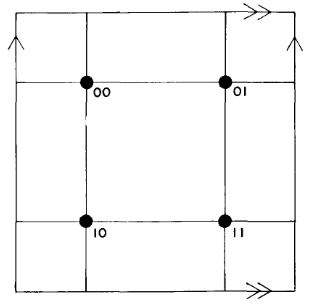
\includegraphics[width=0.5\columnwidth]{figure/rt1.JPG}
\caption{The rectangular toroidal network}
\label{fig:rt1}
\end{figure}

\begin{figure}[!ht]
\centering
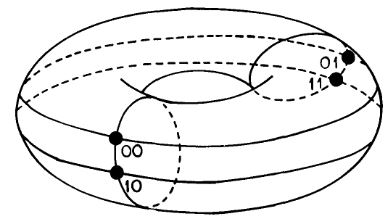
\includegraphics[width=0.5\columnwidth]{figure/rt2.JPG}
\caption{The rectangular toroidal network}
\label{fig:rt2}
\end{figure}
  
\begin{itemize}
\item $m$ : There are $m$ processors on the longitude.
\item $n$ : There are $n$ processors on the latitude.  
\item $L$ : The load injection.  
\item $L_{x}$ : The $L$'s longitude coordinate.  
\item $L_{y}$ : The $L$'s latitude coordinate.  
\item $D_{k}$ : $P_{k}$'s shortest Manhattan distance to $L$.  
\item $D_{k,x}$ : $P_{k}$'s longitude shortest Manhattan distance to $L$.  
\item $D_{k,y}$ : $P_{k}$'s altitude shortest Manhattan distance to $L$.  
\end{itemize}

\begin{empheq}[left=\empheqlbrace]
{align}
D_{k} = D_{k,x} + D_{k,y}\\
D_{k,x} = \min \{\| D_{k,x} - L_{x}\| ,  m - \| D_{k,x} - L_{x}\|\}\\
D_{k,y} = \min \{\| D_{k,y} - L_{y}\| ,  n - \| D_{k,y} - L_{y}\|\}
\end{empheq}
\\
\section{With Front-end Scenario}
\subsection{Data Injection On The Grid Processor}
In $m*n (m = 6,  n = 6)$ \Fig{rt0} toroidal rectangle network, $L$ happens on grid position $(4, 2)$.  We calculate the $D_{k,i}$ table \Tab{rt} by breadth first search(\textbf{\textit{BFS}}) algorithm.  

\begin{figure}[!ht]
\centering
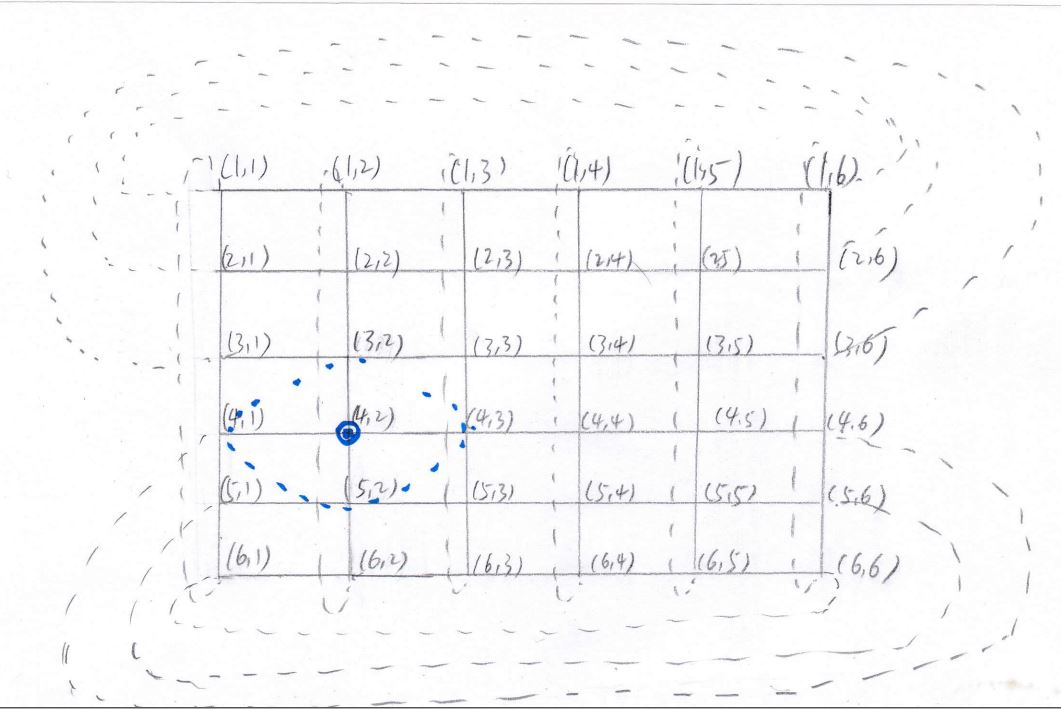
\includegraphics[width=1\columnwidth]{figure/rt0.JPG}
\caption{The m*n toroidal rectangle network and the data injection is $P_{4, 2}$}
\label{fig:rt0}
\end{figure}
\newpage 

The $D_{k,i}$ table is as follow in table \Tab{rt}
\begin{table}
\centering
\small
\setlength\tabcolsep{2pt}
\begin{tabular}{|c|c|}
\hline
    $D_{i}$ & Number\\ 
    \hline
    0 & 1 \\ \hline
    1 & 4 \\ \hline
    2 & 8\\ \hline
    3 & 10\\ \hline
    4 & 8 \\ \hline
    5 & 4 \\ \hline
    6 & 1\\
\hline
\end{tabular}
\caption{$D_{i}$ vs Number}
\label{tab:rt}
\end{table}


The flow matrix closed-form is 

\begin{equation}
{
\left[ \begin{array}{ccccccc}
1 & 4 & 8 & 10 & 8 & 4 & 1\\
1 & -1 & 0 & 0 & 0 & 0 & 0\\
0 & \sigma-1 & 1 & 0 & 0 & 0 & 0\\
0 & \sigma-1 & \sigma & 1 & 0 & 0 & 0\\
0 & \sigma-1 & \sigma & \sigma & 1 & 0 & 0\\
0 & \sigma-1 & \sigma & \sigma & \sigma & 1 & 0\\
0 & \sigma-1 & \sigma & \sigma & \sigma & \sigma & 1\\

\end{array} 
\right ]} \times \left[ \begin{array}{c}
\alpha_{0} \\
\alpha_{1} \\
\alpha_{2} \\
\alpha_{3} \\
\alpha_{4}\\
\alpha_{5}\\
\alpha_{6}\\
\end{array} 
\right ] = \left[ \begin{array}{c}
1 \\
0 \\
0 \\
0 \\
0\\
0\\
0
\end{array} 
\right ]
\end{equation}
\newpage

The simulation result is :

\begin{figure}[!ht]
\centering
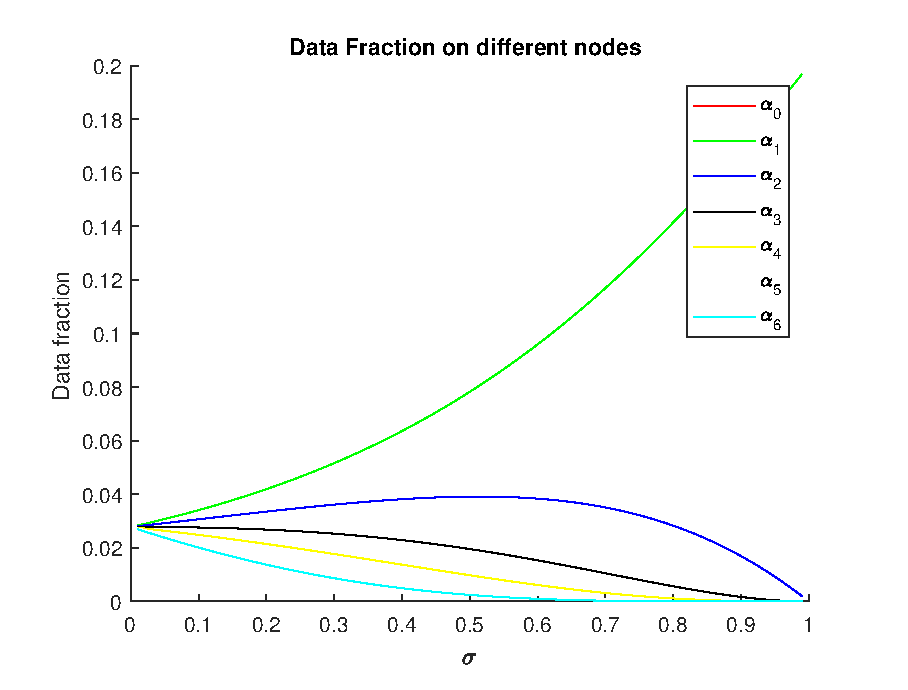
\includegraphics[width=1\columnwidth]{figure/rtfraction.eps}
\caption{The data fraction curve of \Fig{rt0}}
\label{fig:rtfraction}
\end{figure}

From \Fig{rtfraction},  we see that as the value $\sigma$ grows, more and more workload is assigned to the $P_{4, 2}$ and its one hop neighbors.   That is,  as the communication ability decades,  the economical method is to locally process the job.  

The figure illustrates that if $\sigma < 0.3$, the number of processors grow up, the speedup efficiency is likely linear increasing.   Alternatively speaking, if $\sigma < 0.3$, the number of cores dominate the efficiency.   If the $\sigma > 0.3$, the efficiency drops dramatically.   That is, the $\sigma$ value plays more critical role in the speedup simulation.   This important investigation benefit the multi-source assignment problem.   In addition, if the number of cores is bigger than $4$, the bottom speedup effect is about $3$ time.   
\newpage 
\subsection{Sensitivity Analysis of Toroidal Rectangle Network}
Considering a $5*5$ toroidal rectangle network, the $level_{i}$ table shows \Tab{dn}:
\begin{table}
\centering
\small
\setlength\tabcolsep{2pt}
\begin{tabular}{|c|c|}
\hline
    $D_{i}$ & Number\\ 
    \hline
    0 & 1 \\ \hline
    1 & 4 \\ \hline
    2 & 8\\ \hline
    3 & 8\\ \hline
    4 & 4 \\ \hline
\end{tabular}
\caption{The processor number of various $D_{i}$}
\label{tab:dn}
\end{table}

So the simulation result illustrates in \Fig{sa5t5_torus}
\begin{figure}[!ht]
\centering
\includegraphics[width=1\columnwidth]{figure/sa5t5_torus.eps}
\caption{Sensitivity analysis result of data injection position on inner grid processor}
\label{fig:sa5t5_torus}
\end{figure}
\subsection{Multi-source Even Data Injection}
\newpage
\Fig{how_voronoi} \cite{grima2013computational} provides a torus Voronoi method, which extends the original domain to $8$ copy and calculate the Voronoi Diagram as planner algorithm \cite{fortune1987sweepline}.  Then the corner part is the torus Voronoi diagram.

\begin{figure}[!ht]
\centering
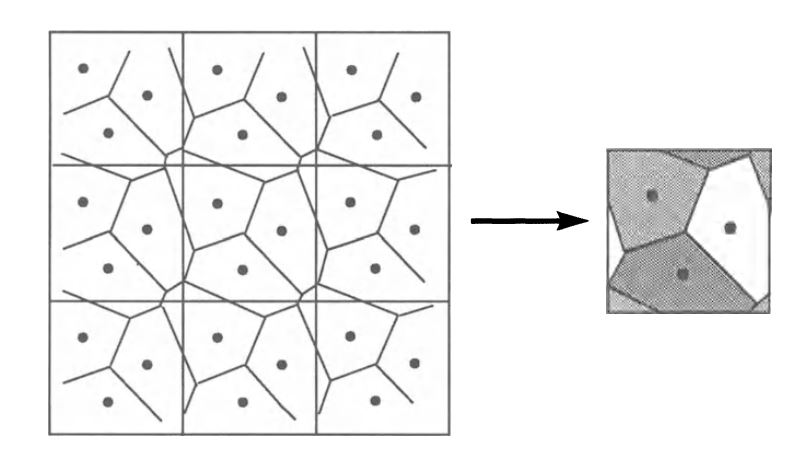
\includegraphics[width=1\columnwidth]{figure/how_voronoi.JPG}
\caption{How to calculate torus Voronoi Diagram}
\label{fig:how_voronoi}
\end{figure}

\begin{figure}[!ht]
\centering
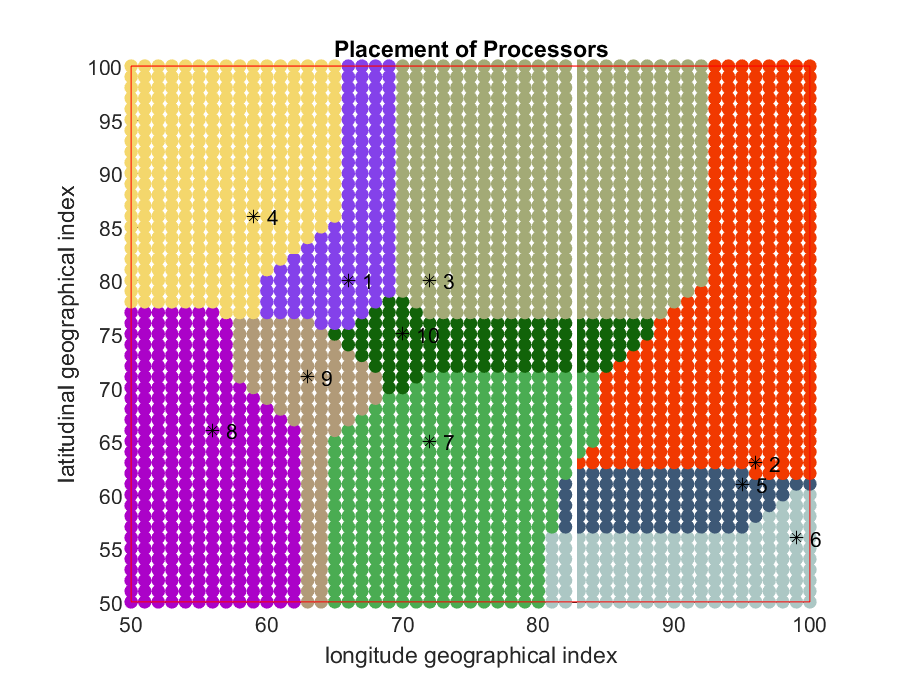
\includegraphics[width=1\columnwidth]{figure/t_1.eps}
\caption{Initial Voronoi Digram}
\label{fig:t_1}
\end{figure}

\begin{figure}[!ht]
\centering
\includegraphics[width=1\columnwidth]{figure/t_voronoi.eps}
\caption{Torus Voronoi Diagram}
\label{fig:t_voronoi}
\end{figure}

\begin{figure}[!ht]
\centering
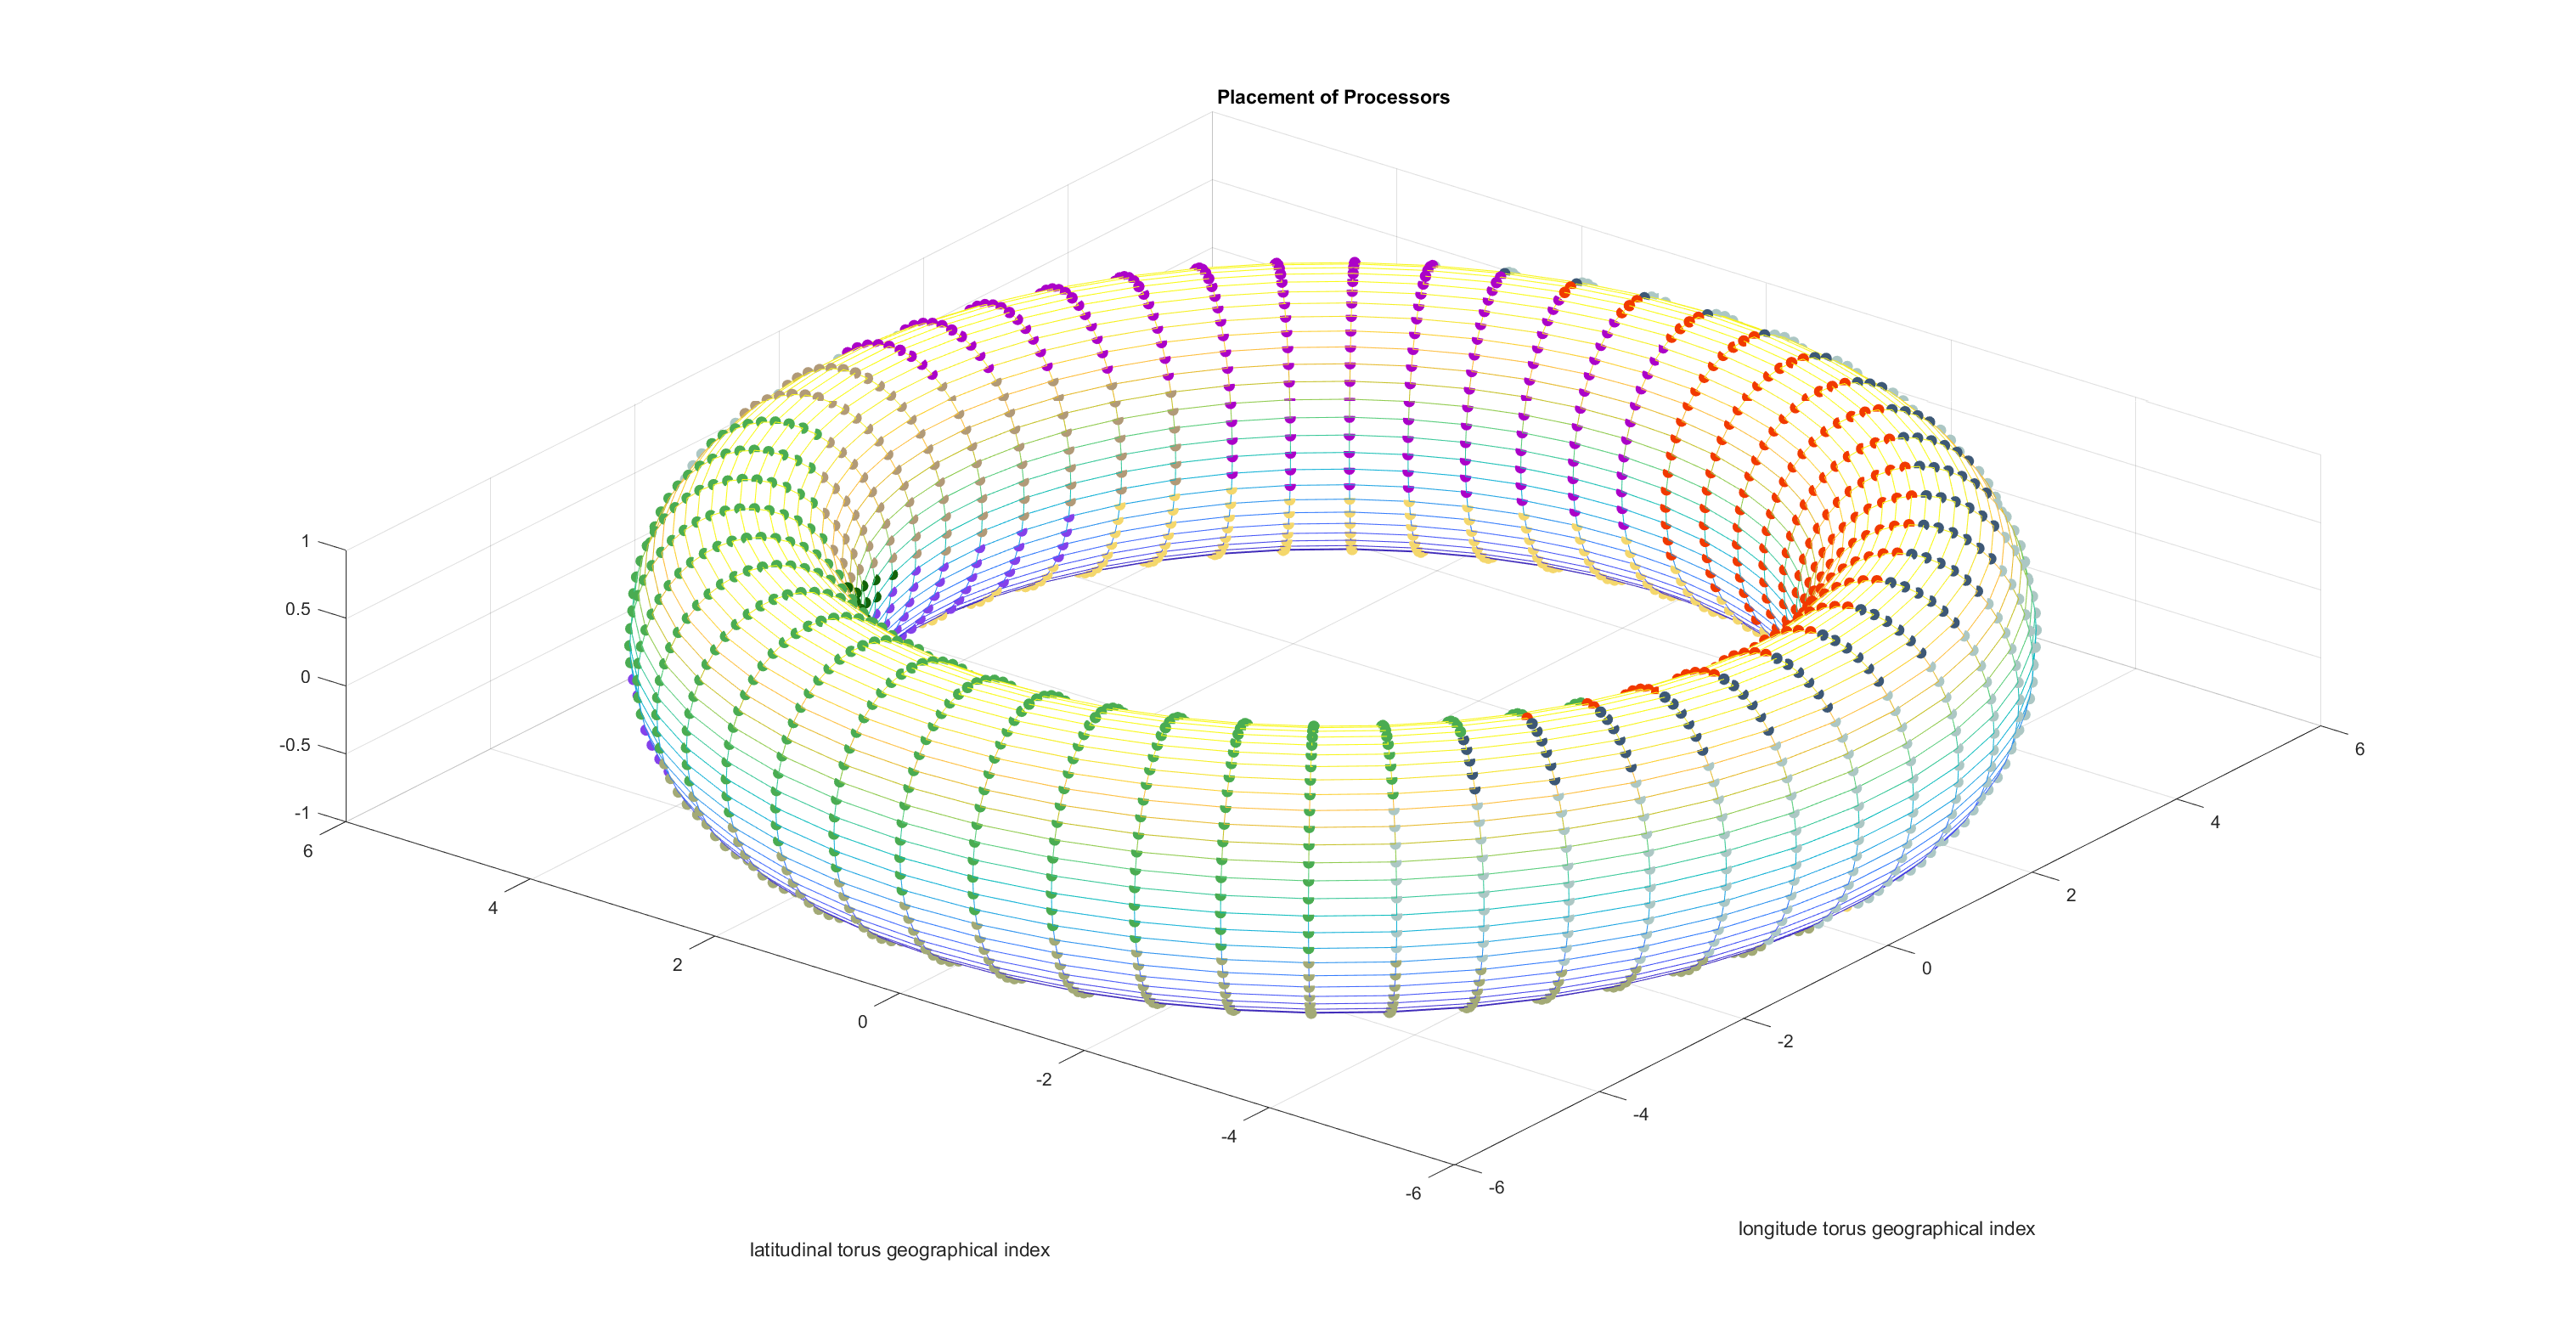
\includegraphics[width=1\columnwidth]{figure/t_voronoi_torus.eps}
\caption{Voronoi Diagram Casting to the torus model}
\label{fig:t_voronoi_torus}
\end{figure}

\begin{figure}[!ht]
\centering
\includegraphics[width=1\columnwidth]{figure/t_voronoi_speedup.eps}
\caption{Voronoi Diagram Casting to the torus model}
\label{fig:t_voronoi_speedup}
\end{figure}
\newpage

In the reduced model, reduced toroidal Voronoi diagram save $27\%$ processors hit the same processing capacity.  The ratio of original method is about $\frac{490}{98} = 5$, after the reduced action, the ratio is $\frac{290}{98} \approx 2.96 $ . That is the reduced heuristic algorithm obtaining more balanced computation capacity distribution.

\begin{figure}[!ht]
\centering
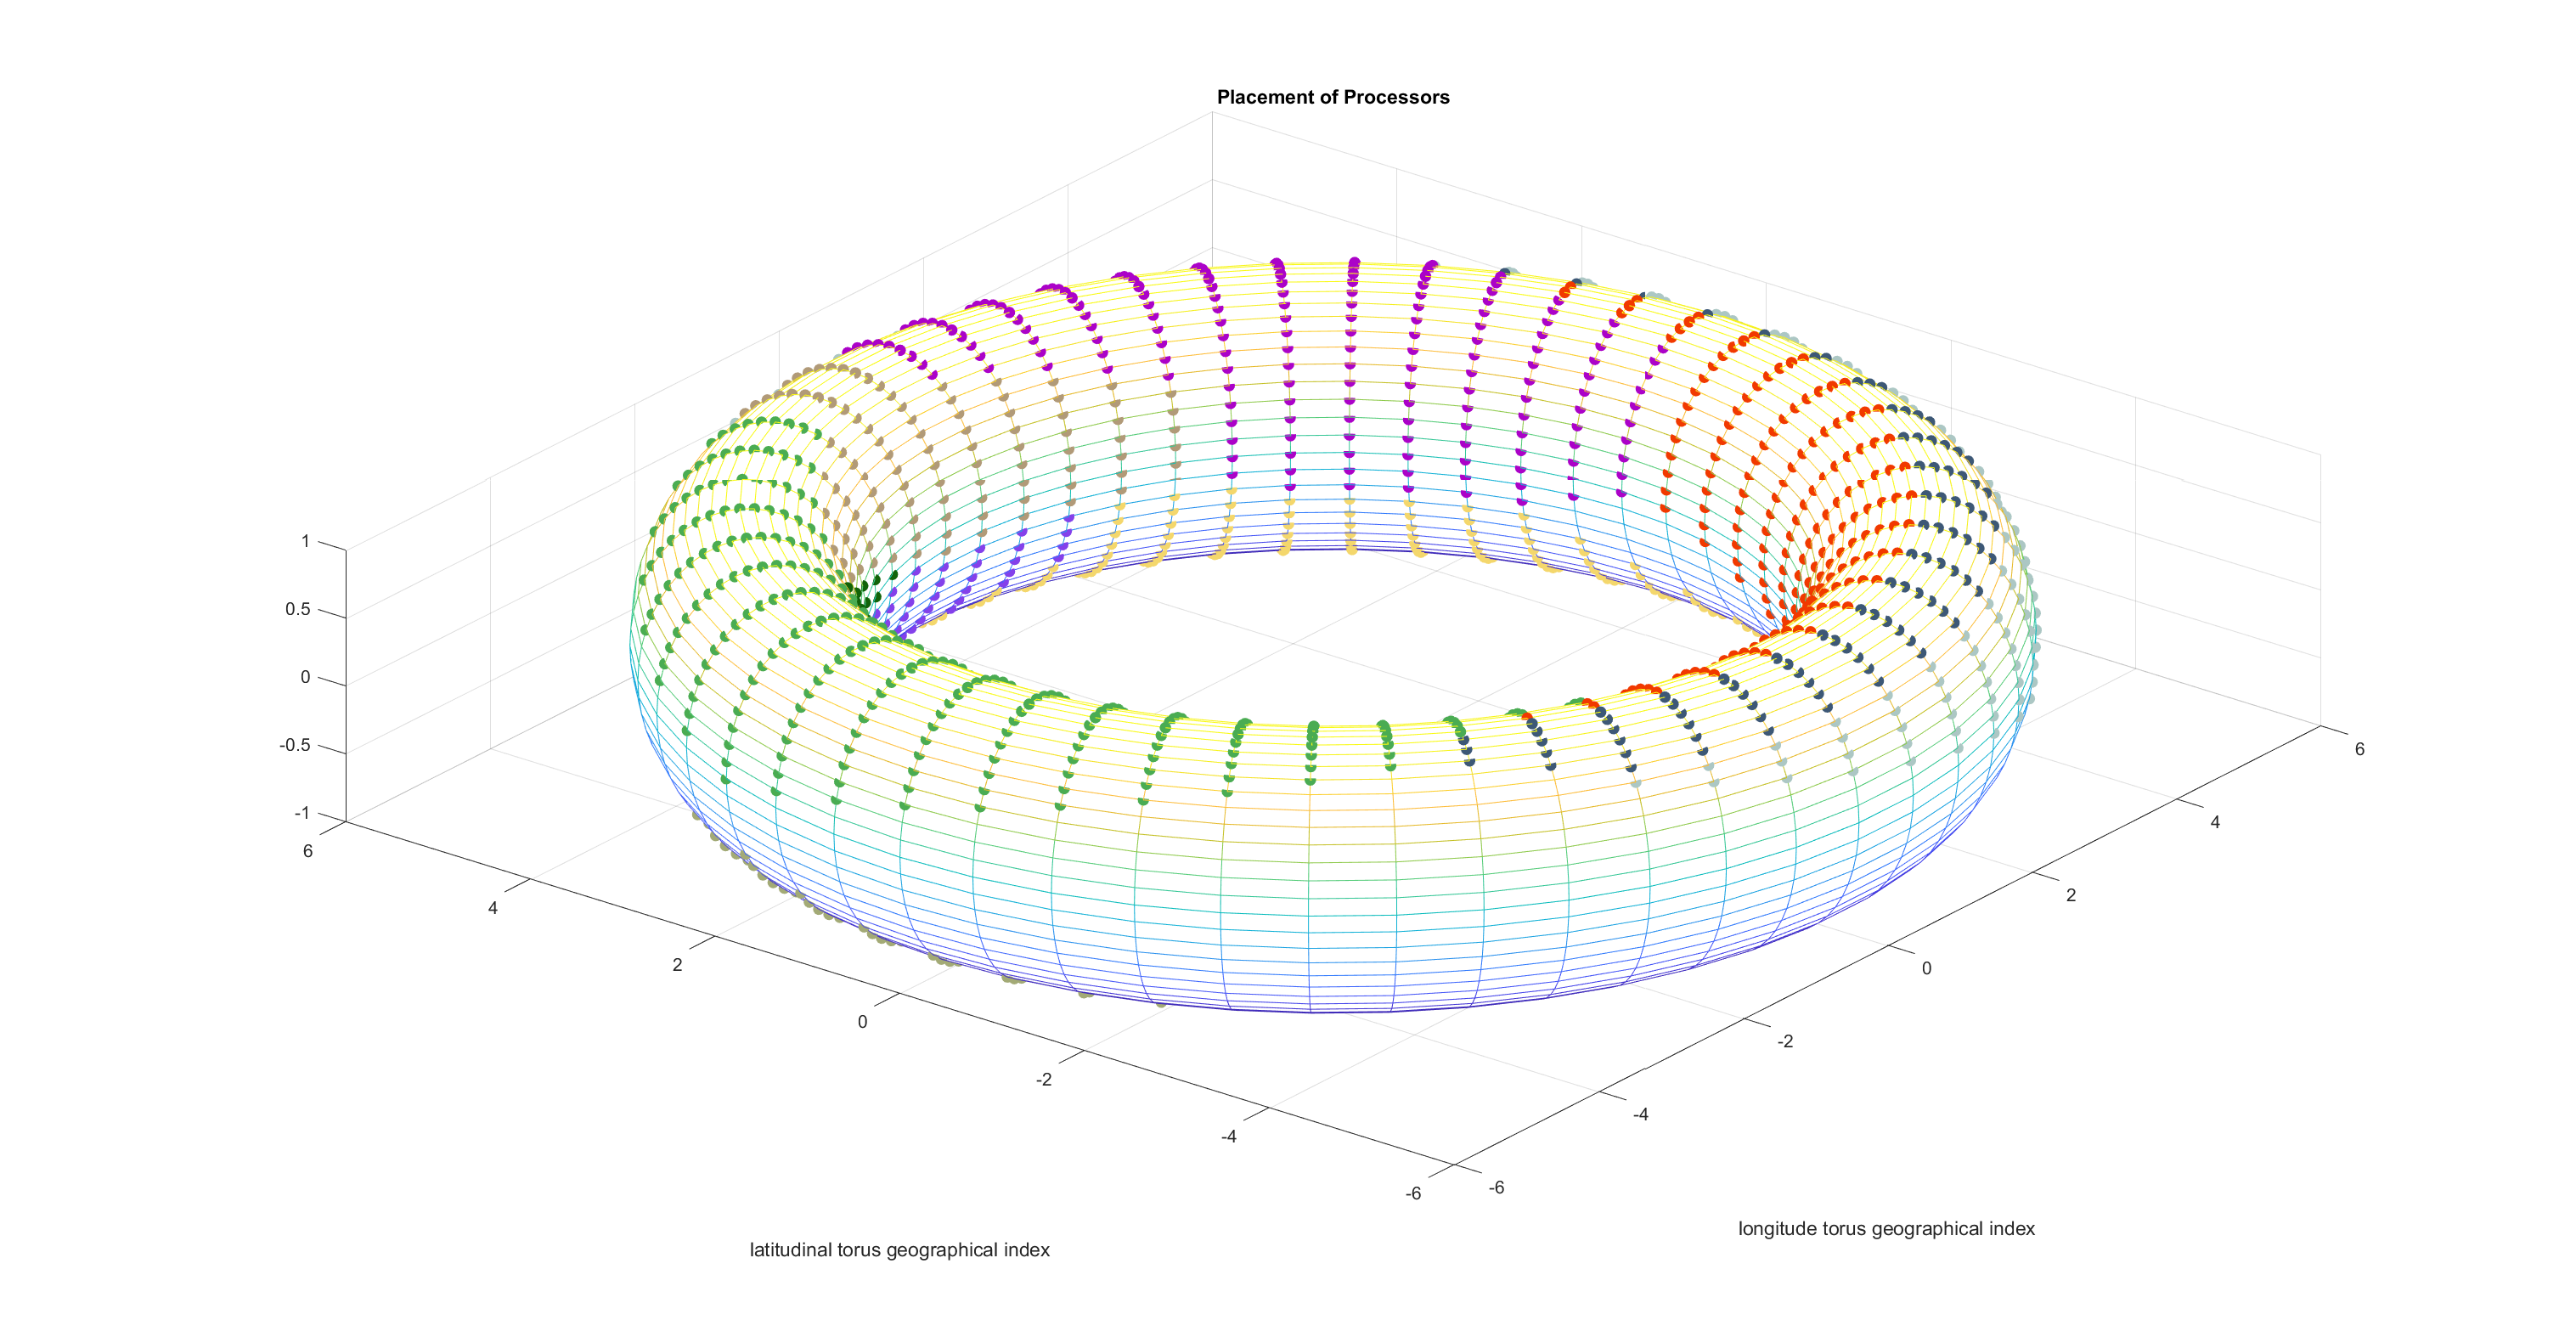
\includegraphics[width=1\columnwidth]{figure/t_voronoi_torus_save.eps}
\caption{Torus Reduced Voronoi Diagram Casting to the Torus Model}
\label{fig:t_voronoi_torus_save}
\end{figure}

\begin{figure}[!ht]
\centering
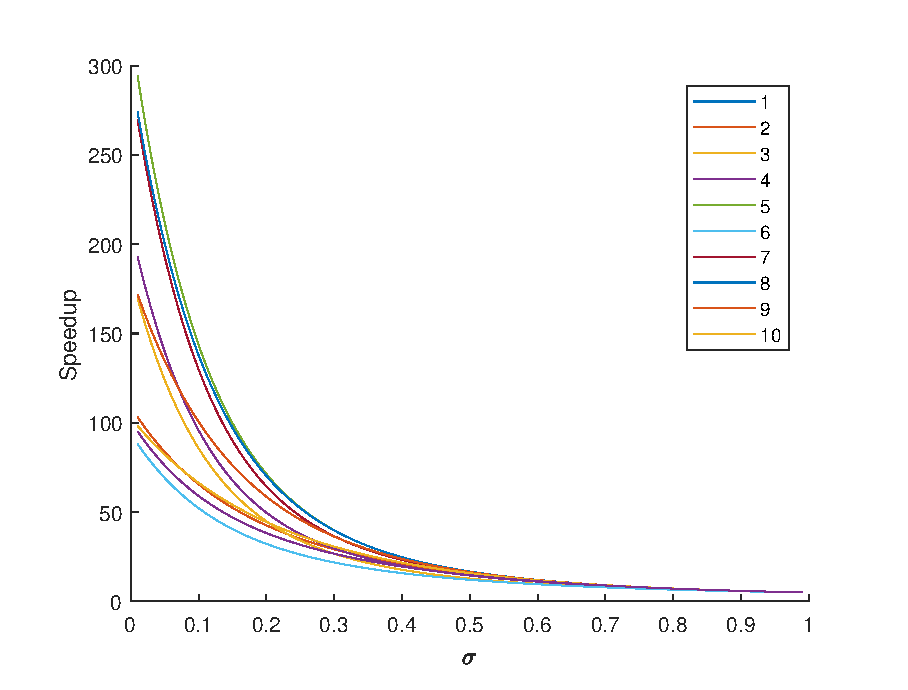
\includegraphics[width=1\columnwidth]{figure/t_voronoi_speedup_save.eps}
\caption{Torus Reduced Voronoi Diagram}
\label{fig:t_voronoi_speedup_save}
\end{figure}


\subsection{Multi-source Different Data Injection}
\newpage


\section{Without Front-end Scenario}
\subsection{Data Injection On The Grid Processor}
We utilize the $\sigma^{\star}$ to present $-(\sigma+1)$.  
The flow matrix closed-form of \Fig{rt0} is:
\begin{equation}
{
\left[ \begin{array}{ccccccc}
1 & 4 & 8 & 10 & 8 & 4 & 1\\
1 & \sigma^{\star} & 0 & 0 & 0 & 0 & 0\\
1 & -\sigma & \sigma^{\star} & 0 & 0 & 0 & 0\\
1 & -\sigma & -\sigma & -\sigma^{\star} & 0 & 0 & 0\\
1 & -\sigma & -\sigma & -\sigma & \sigma^{\star} & 0 & 0\\
1 & -\sigma & -\sigma & -\sigma & -\sigma & \sigma^{\star} & 0\\
1 & -\sigma & -\sigma & -\sigma & -\sigma & -\sigma & \sigma^{\star}
\end{array} 
\right ]} \times \left[ \begin{array}{c}
\alpha_{0} \\
\alpha_{1} \\
\alpha_{2} \\
\alpha_{3} \\
\alpha_{4}\\
\alpha_{5}\\
\alpha_{6}\\
\end{array} 
\right ] = \left[ \begin{array}{c}
1 \\
0 \\
0 \\
0 \\
0\\
0\\
0
\end{array} 
\right ]
\end{equation}
The fraction curve result is :

\begin{figure}[!ht]
\centering
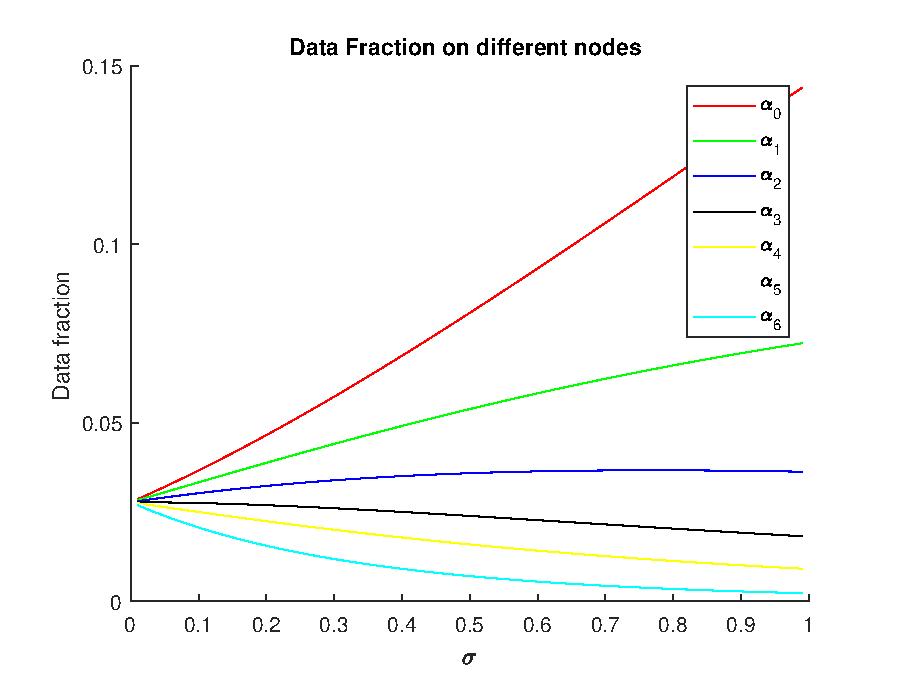
\includegraphics[width=1\columnwidth]{figure/rt_no_fraction.eps}
\caption{The data fraction curve of \Fig{rt0} }
\label{fig:rt_no_fraction}
\end{figure}

From \Fig{rt_no_fraction},  we see that as the value $\sigma$ grows, more and more workload is assigned to the $P_{4, 2}$ and its one hop neighbors.   That is,  as the communication ability decades,  the economical method is to locally process the job. 
\newpage
\subsection{Sensitivity Analysis of Toroidal Rectangle Network}
Considering a $5*5$ toroidal rectangle network, the $level_{i}$ table shows \Tab{dn_2}:
\begin{table}
\centering
\small
\setlength\tabcolsep{2pt}
\begin{tabular}{|c|c|}
\hline
    $D_{i}$ & Number\\ 
    \hline
    0 & 1 \\ \hline
    1 & 4 \\ \hline
    2 & 8\\ \hline
    3 & 8\\ \hline
    4 & 4 \\ \hline
\end{tabular}
\caption{The processor number of various $D_{i}$}
\label{tab:dn_2}
\end{table}

So the simulation result illustrates in \Fig{sa5t5_torus_no}
\begin{figure}[!ht]
\centering
\includegraphics[width=1\columnwidth]{figure/sa5t5_torus.eps}
\caption{Sensitivity analysis result of data injection position on inner grid processor}
\label{fig:sa5t5_torus_no}
\end{figure}
\newpage
\subsection{Multi-source Even Data Injection}
\newpage
\subsection{Multi-source Different Data Injection}
\newpage

\section{Comparison Result}
\subsection{Comparison Result Between Regular Mesh and Toroidal With Same Processors Number}
Considering a regular mesh \Fig{5t5}, the best position for data injection is $P_{12}$.   Other positions, for example $P_{8}$, $P_{13}$, they don't have the same speedup efficiency.   Yet, for a toroidal $5*5$ regular mesh, each position's efficiency is equal.  \Fig{sacom5t5ci} explores the comparison result between the toroidal and corner scenario difference. 

\subsection{Comparison Result With Corner Processor and Inner Grid Processor}
For a $5*5$ regular network, the inner grid position is $P_{12}$ and the corner data injection position is $P_{0}$.  
The comparing result is \Fig{sacom5t5ci}.  

\begin{figure}[!ht]
\centering
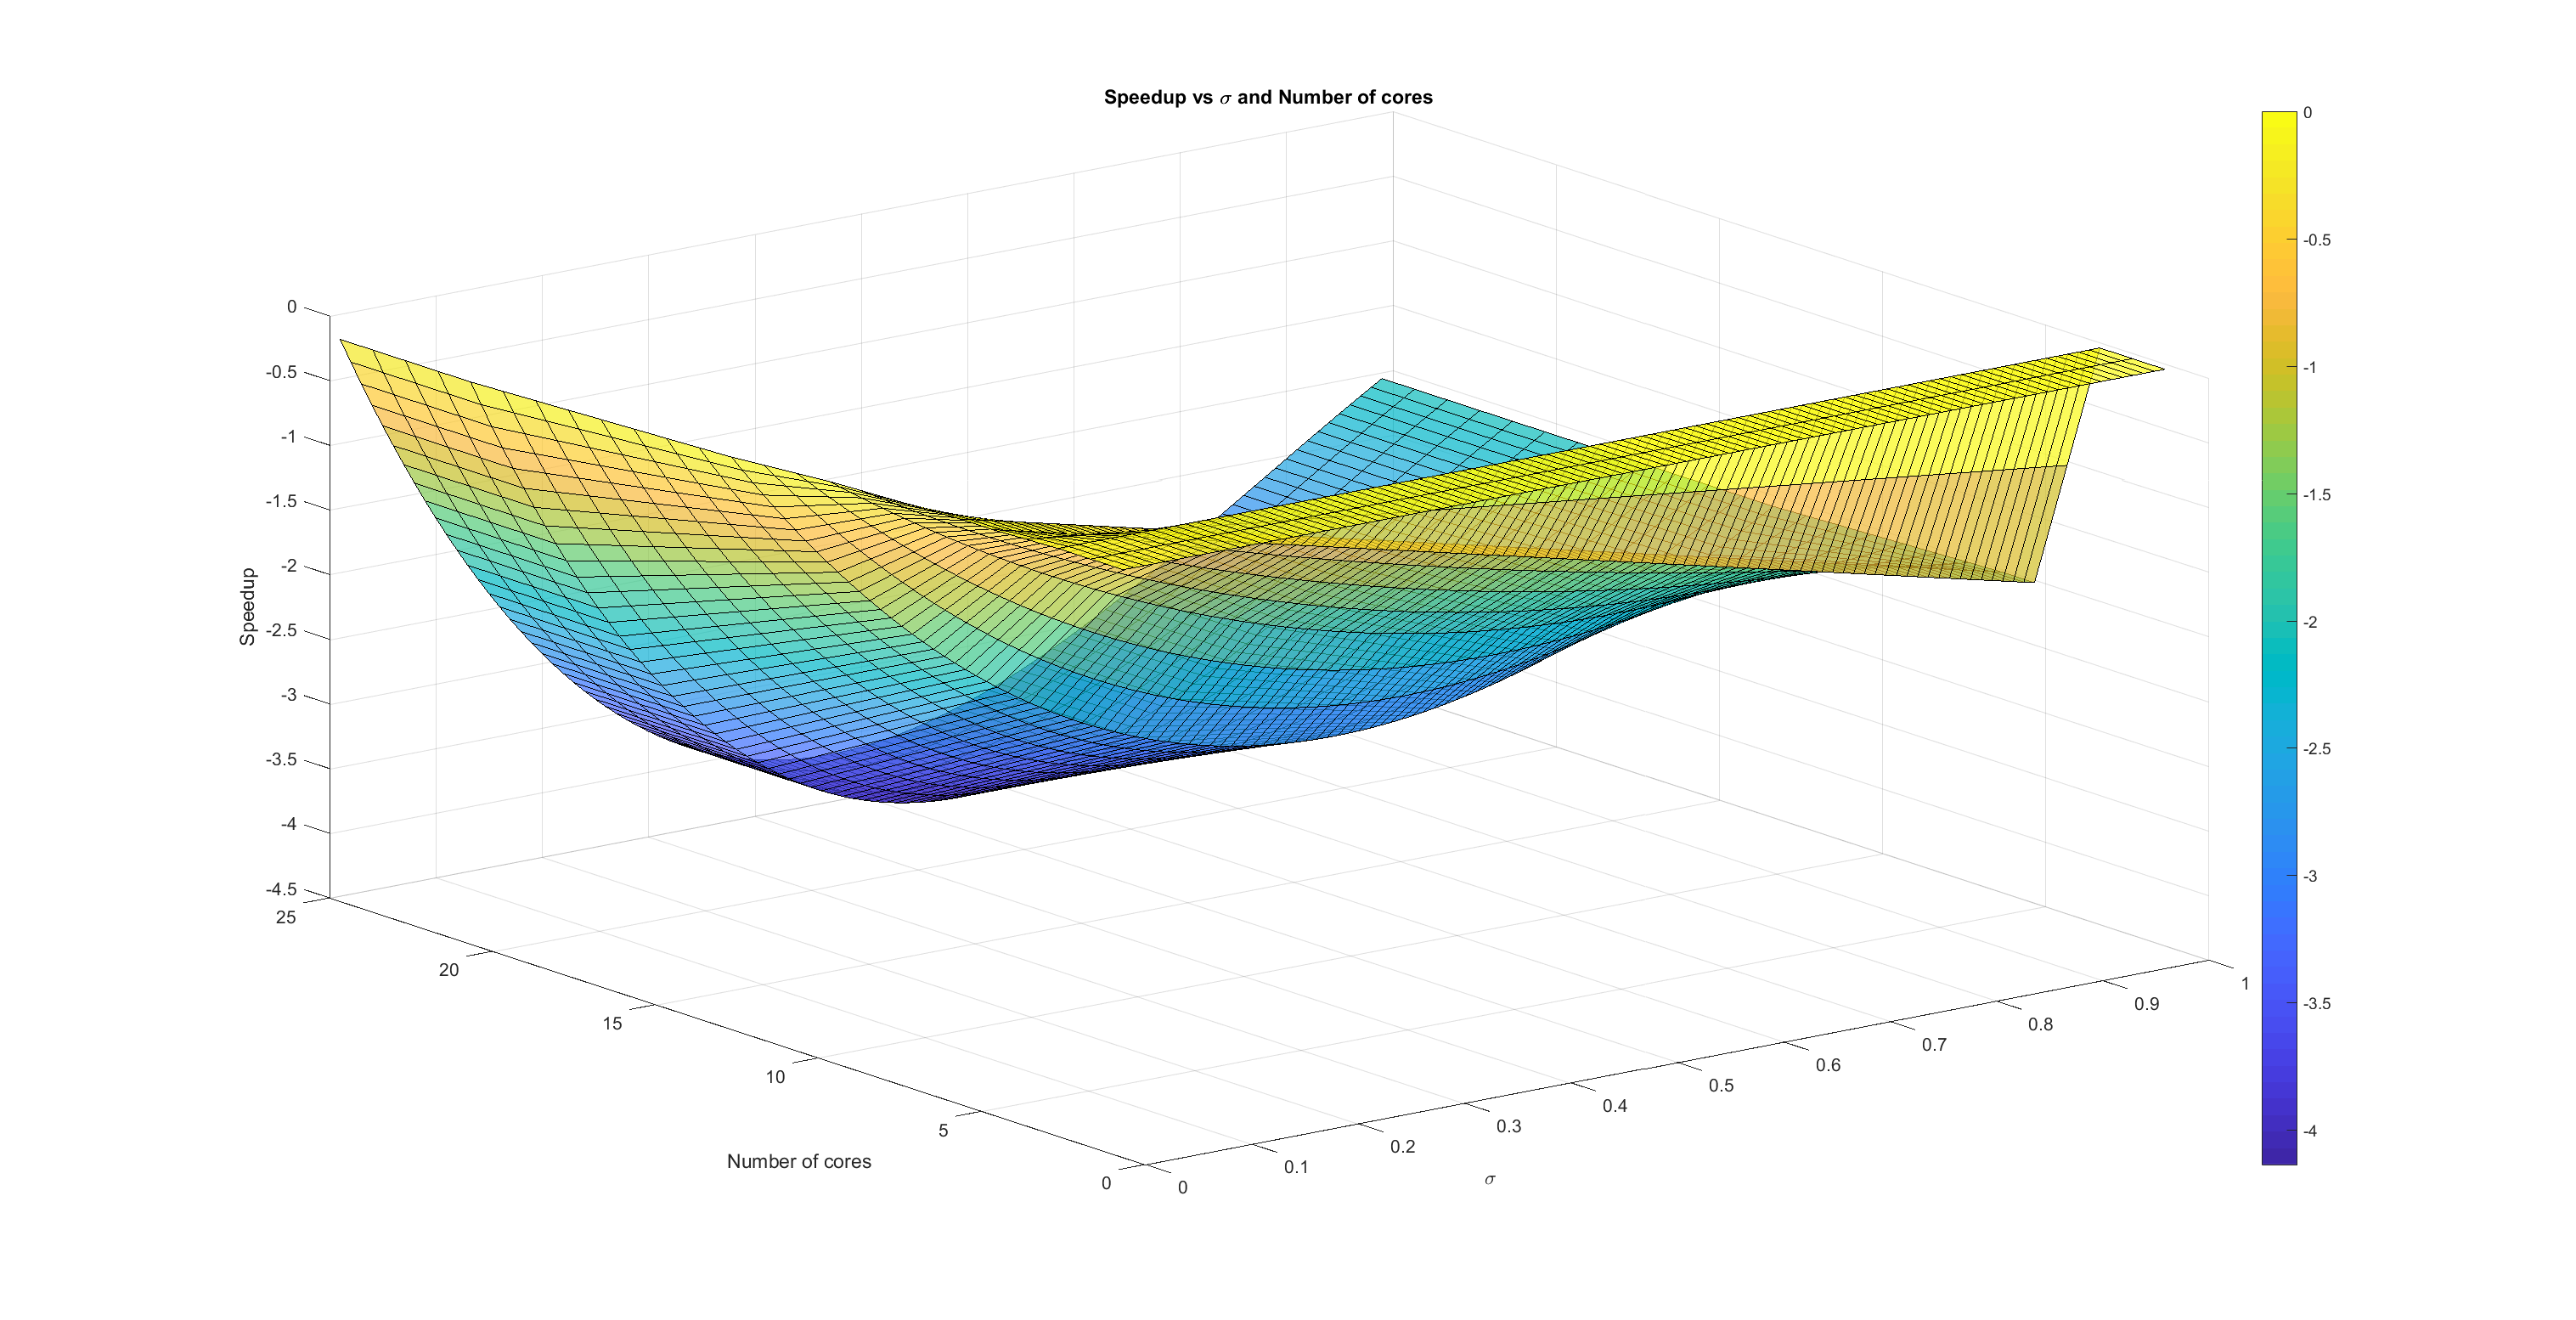
\includegraphics[width=1\columnwidth]{figure/sacom5t5ci.eps}
\caption{ Speedup difference between corner injection and inner grid injection}
\label{fig:sacom5t5ci}
\end{figure}

Generally speaking, \Fig{sacom5t5ci} says the inner grid position scenario has better performance than the corner injection option.   If the grid node is $25$ and $\sigma = 0.5$, the speedup difference is largest, which is $4$.  
\newpage

\subsection{Comparison Result Between Front-end Processor and Without Front-end Processor}

In the legend of figures,  we use 
\begin{itemize}
\item $F$ presents the processors are with front-end situation.
\item $NF$ presents the processors are without front-end situation.
\item $F\alpha_{0}$ means the $\alpha_{0}$ data fraction deployed to $P_{0}$, if the processor has front-end.
\item $NF\alpha_{0}$ means the $\alpha_{0}$ data fraction deployed to $P_{0}$, if the processor is without front-end setting.
\end{itemize}

\subsubsection{Data Injection On the Corner Processor}

\begin{figure}[!ht]
\centering
\includegraphics[width=1\columnwidth]{figure/2t2_c.eps}
\caption{The comparing result between front-end processor with without front-end processor in 2*2 regular network }
\label{fig:2t2_c}
\end{figure}

\Fig{2t2_c} says that $P_{0}$ takes more assigned task in without front-end scenario than front-end processor situation.  As the value $\sigma$ value goes up, the fractions are deployed to the deeper layers decreases.  In the limit condition, for example, $\sigma  = 1$,  there is no data transmitted to $P_{3}$ in the front-end assumption,  yet in the without front-end situation,  there is still about $10\%$ data fraction are communicated to $P_{3}$.  
\newpage

\begin{figure}[!ht]
\centering
\includegraphics[width=1\columnwidth]{figure/2t3_c.eps}
\caption{The comparing result between front-end processor with without front-end processor in 2*3 regular network }
\label{fig:2t3_c}
\end{figure}
\newpage

\Fig{2t3_c} says that $P_{0}$ takes more assigned task in without front-end scenario than front-end processor situation.  As the $\sigma$ value goes up, the fractions are deployed to the deeper levels degrades.  In the limit condition, for example, $\sigma  = 1$,  there is no data transmitted to $level_{3}$, that is, $P_{5}$ in the front-end assumption.  Yet in the without front-end situation,  there is still about $5\%$ data fraction is communicated to $P_{5}$.  
\newpage 

\begin{figure}[!ht]
\centering
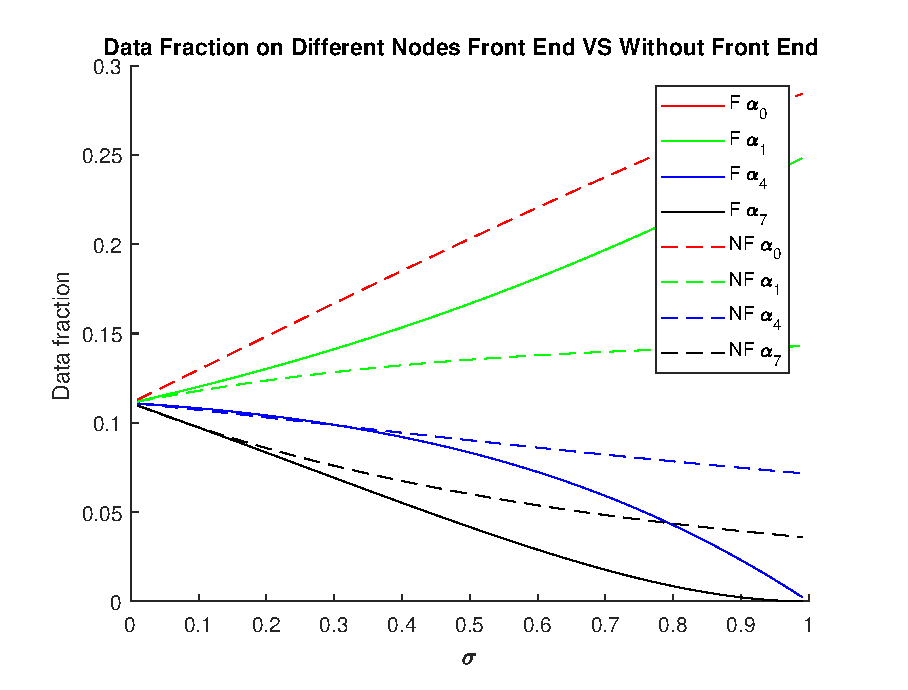
\includegraphics[width=1\columnwidth]{figure/3t3b_c.eps}
\caption{The comparing result between front-end processor with without front-end processor in 3*3 regular network injection on boundary processor }
\label{fig:3t3b_c}
\end{figure}

\Fig{3t3b_c} says that $P_{0}$ takes more assigned task in without front-end scenario than front-end processor situation.  As the $\sigma$ value goes up, the fractions are deployed to the deeper levels decreases.  In the limit condition, for example, $\sigma  = 1$,  there is no data transmitted to $level_{3}$, that is, $P_{7}$ and $P_{8}$ in the front-end assumption.  Yet in the without front-end situation,  there is still about $5\%$ data fraction is communicated to $P_{7}$ and $P_{8}$.  

\newpage 
\begin{figure}[!ht]
\centering
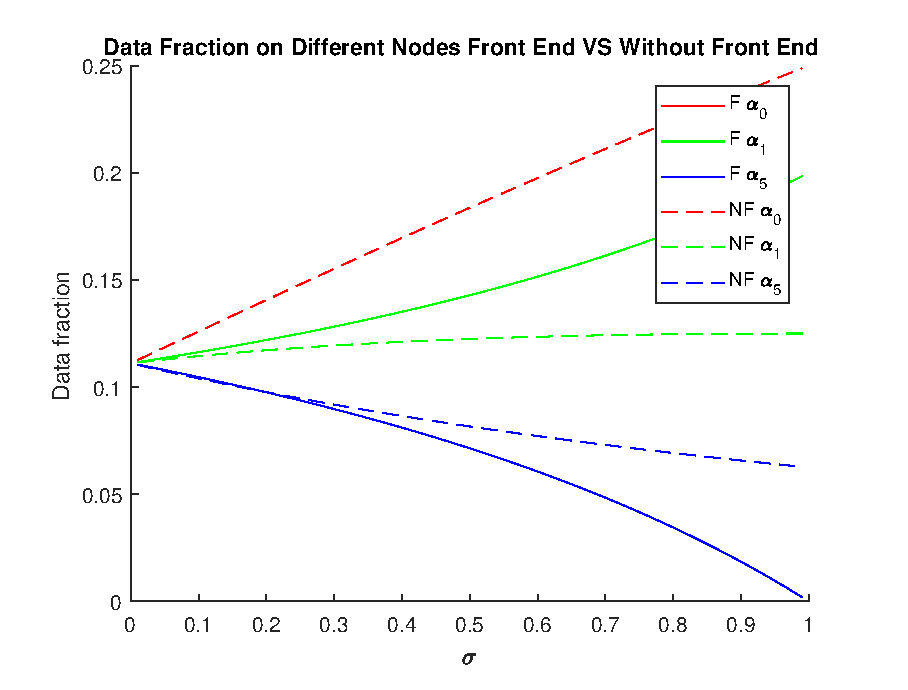
\includegraphics[width=1\columnwidth]{figure/3t3i_c.eps}
\caption{The comparing result between front-end processor with without front-end processor in 3*3 regular network injection on inner grid processor }
\label{fig:3t3i_c}
\end{figure}

\Fig{3t3i_c} says that $P_{0}$ takes more assigned task in without front-end scenario than front-end processor situation.  As the $\sigma$ value goes up, the fractions are deployed to the deeper levels dropping down.  In the limit condition, for example, $\sigma  = 1$,  there is no data transmitted to $level_{2}$, that is, $P_{5}$, $P_{6}$, $P_{7}$ and $P_{8}$ in the front-end assumption.  Yet in the without front-end situation,  there is still about $5\%$ data fraction is communicated to $P_{5}$, $P_{6}$, $P_{7}$ and $P_{8}$.  

Comparing with \Fig{3t3b_c}, $P_{0}$ takes less workload in inner grid position than boundary data injection.  The reason is there are 4 neighbor processors on the $level_{1}$, yet there is solely three processors on $level_{1}$ on the boundary.
\newpage 

\begin{figure}[!ht]
\centering
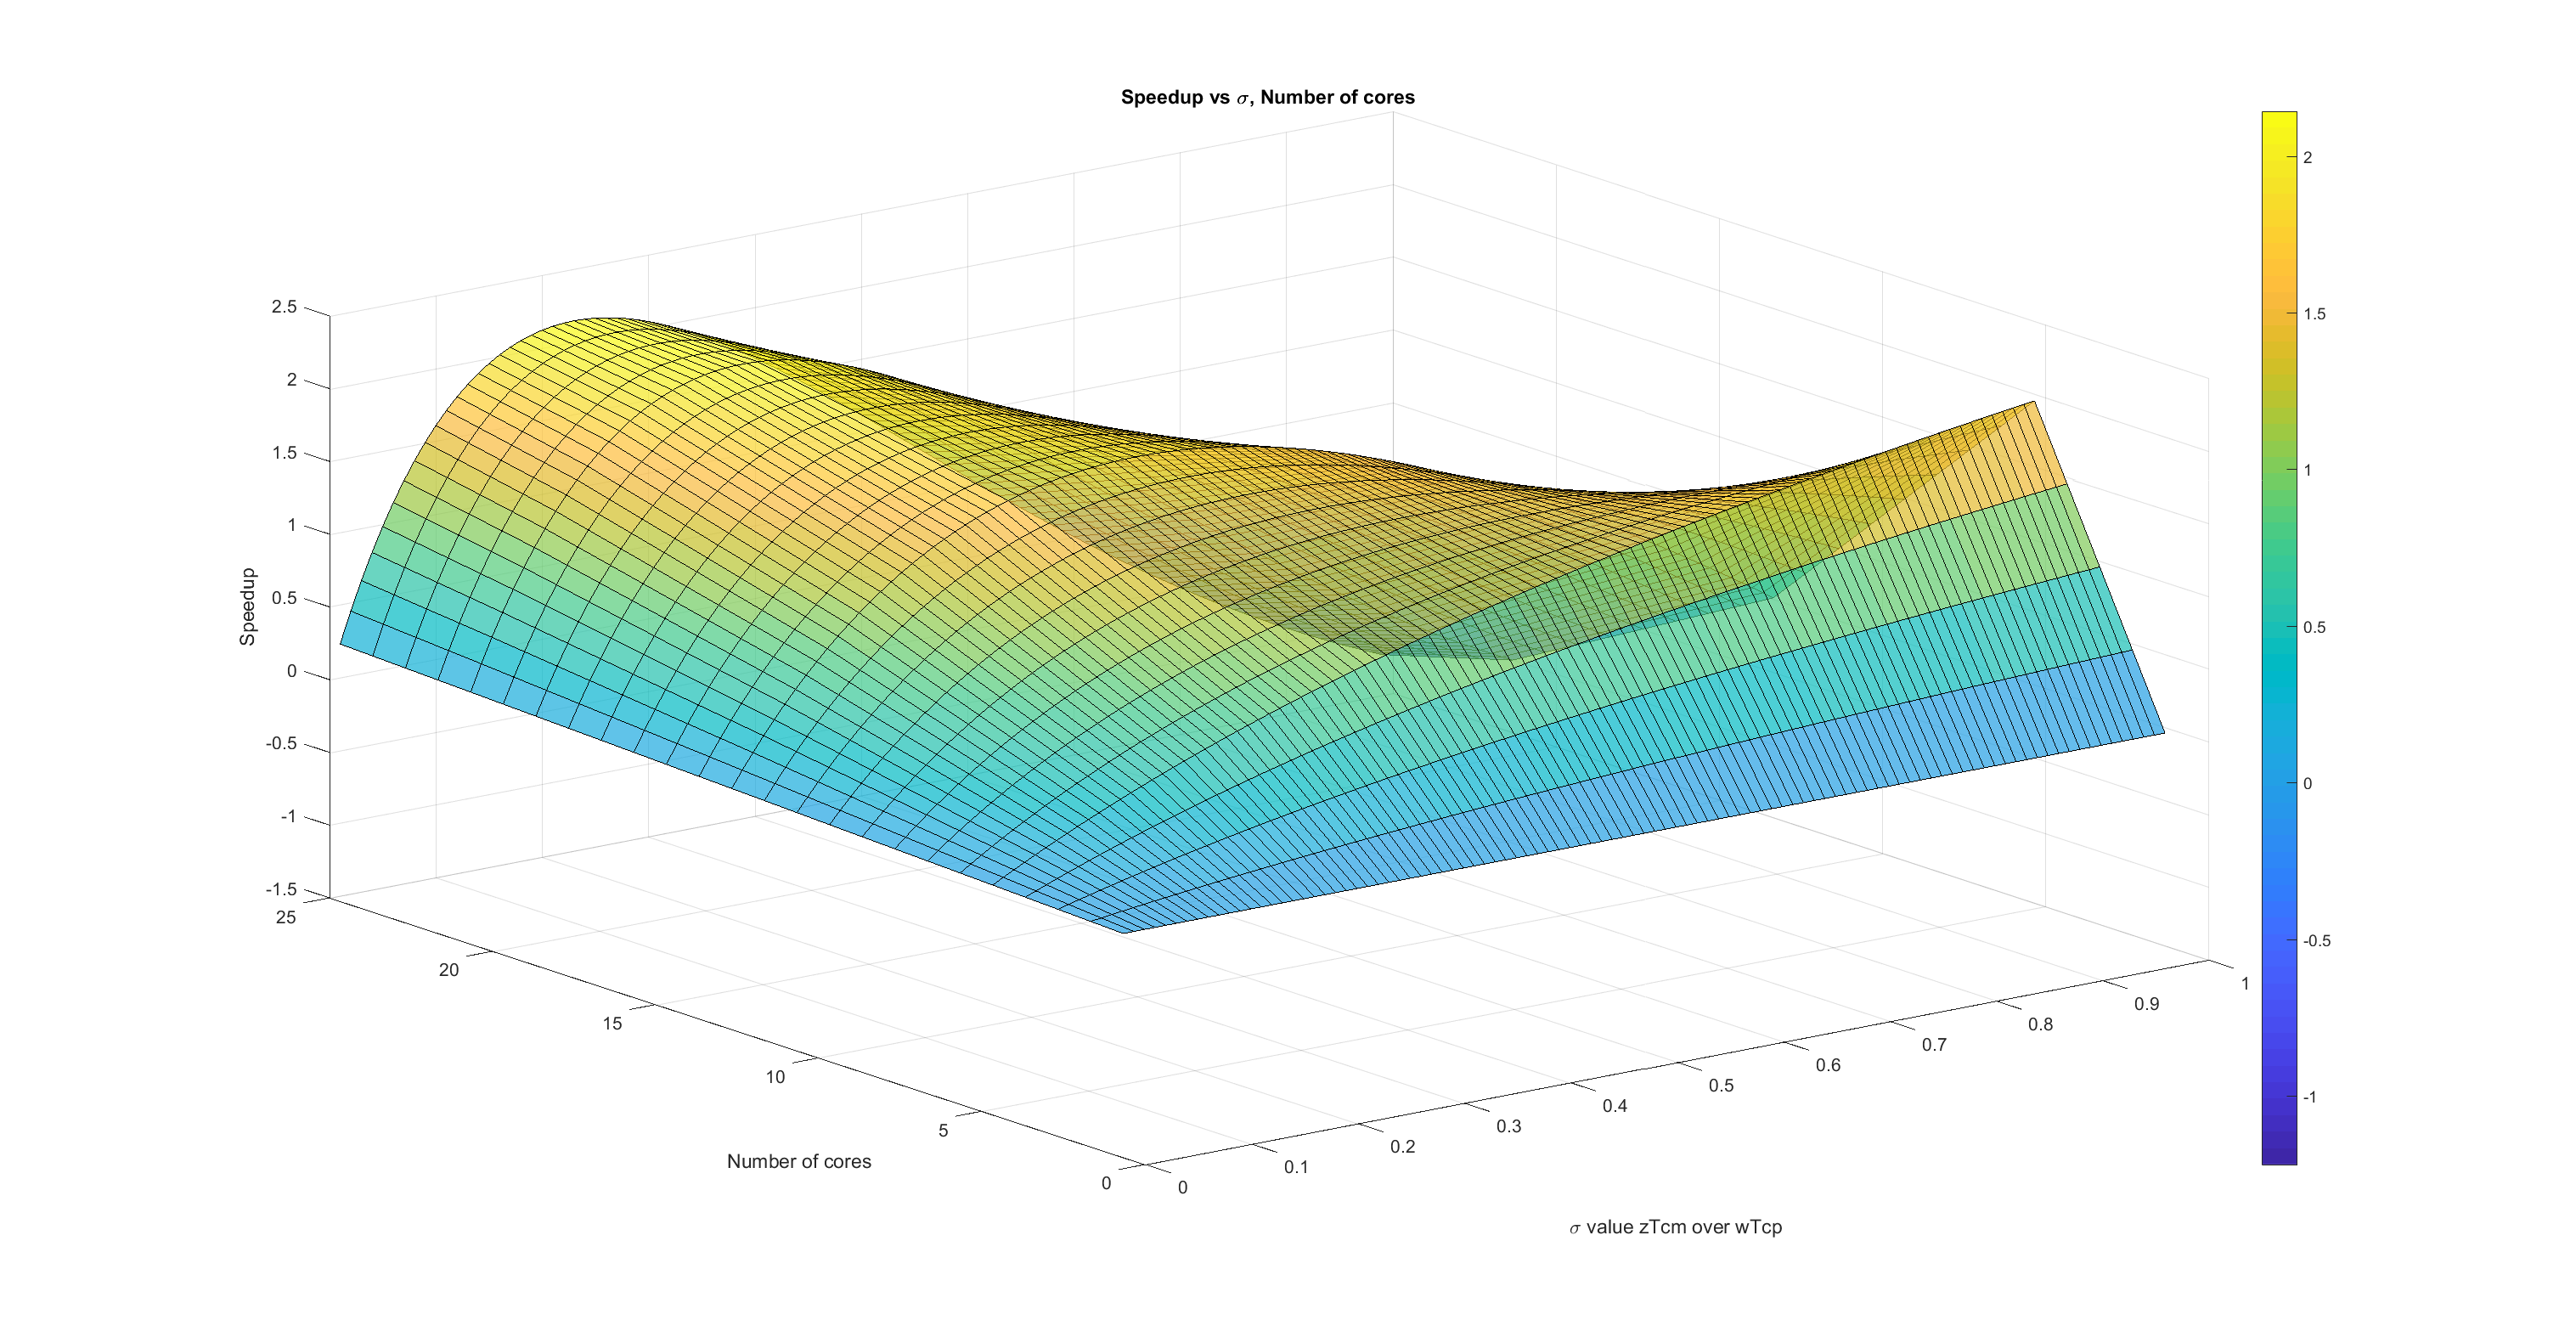
\includegraphics[width=1\columnwidth]{figure/sacom5t5f_nof.eps}
\caption{ Speedup difference between front-end and without front-end in 5*5 regular network}
\label{fig:sacom5t5f_nof}
\end{figure}

\Fig{sacom5t5f_nof} shows the speedup difference between the front-end situation and without front-end scenario.  


\newpage
\section{Store and Froward Switching}
In this chapter, we mainly discuss the virtual cut through \cite{kermani1979virtual} switching.  In addition, the store and froward \cite{kanthraj2007store} schema is a mature data processing technique.  In future works, we discuss it.



